\documentclass[12pt,a4paper]{article}
\title{\textsc{COS 332 - Practical 1 Answers}}
\author{\textsc{R.R. Koopmans, 15043143}}
\usepackage{graphicx}

\begin{document}
\maketitle

\paragraph{Question 1}

\texttt{traceroute} itself cannot tell us why this is happening.
\texttt{traceroute} can only relay information from packets that are returned to
the sender. If packets are rejected, these appear as a ``\textbf{*}'', and the fact
that the packet was not returned is all the information we can draw from this
outcome. It may be that the domain does not exist, or a firewall has blocked the
connection, or a connection was interrupted. We cannot know whether is was any
one of these, or even a combination.

Fortunately the answer for outcome is explainable through extra information.
This is because all domains on the UP network are registered under the
\texttt{137.215.XXX.XXX} address prefix. This means that the address 8.8.8.8
does not exist in the scope of this subnet and can hence not be traced to.

\paragraph{Question 2}

No, you cannot trace the route to \texttt{up.ac.za} from campus. This is because
this domain is not hosted locally on the university network. This is
demonstrated by the fact that when you try to \texttt{traceroute} to the domain
we see one final SYN packet to a domain outside the network, which  is never
acknowledged (i.e. no ACK is sent in return). This means that the packet has
been refused by the university firewall and access has been denied to this
outside

\paragraph{Question 3}

\begin{center}
  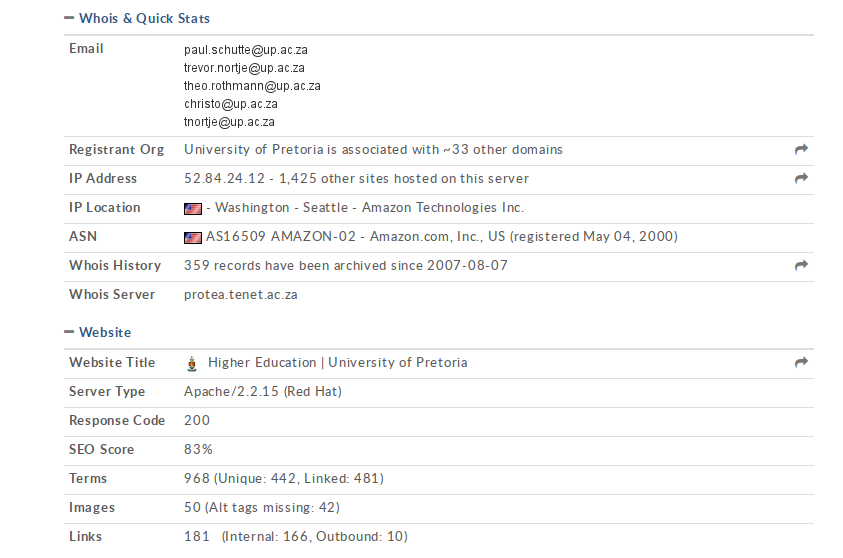
\includegraphics[scale=0.5]{whoiscropped}
\end{center}

\end{document}
